
\begingroup
\hspace{4.5mm}
\setlength{\parindent}{0pt}


\section*{Termo de Aceite de Contrato de Prestação de Serviços}
\subsection*{Identificação das Partes}

\textbf{Contratante:}\\

\begingroup

    \leftskip 20pt
    \rightskip 20pt
    
    Nome: Mangaba’s Kitchen\\
    Endereço: Salvador-BA\\
    Representante Legal: Mateus de Jesus\\\\

\endgroup

\textbf{Contratada:}\\

\begingroup

    \leftskip 20pt
    \rightskip 20pt
    
    Nome: Mangaba Tech\\
    Endereço: Salvador-BA\\
    Representante Legal: Victor Dantas

\endgroup

\subsection*{Identificação do Programa de Computador (Software)}
Denominação: Sistema de Gerenciamento de Restaurante Mangaba's Kitchen\\\\
Módulo (Objeto): 1 (Uma) cópia do software executável, com licença para uso em tablets para os garçons, em um computador pessoal para o gerente e em uma televisão sensível ao toque para a equipe da cozinha.\\

\subsection*{Requisitos e Funcionalidades}

\leftskip 0pt
\rightskip 0pt
\textbf{I. Objeto.}\\
O presente termo de concordância tem como objetivo validar os requisitos acordados entre as partes para o desenvolvimento do software de gerenciamento de restaurante. O sistema será utilizado para automação de vendas, controle de estoque, gestão de pedidos e geração de relatórios financeiros.\\

\begingroup

    \leftskip 20pt
    \rightskip 20pt
    
    § 1º – A Contratante concorda que o software inclui funcionalidades para gerenciamento de pedidos, como estimativa de tempo de preparo, atualização dos status dos pedidos e consulta ao histórico de pedidos.\\\\
    § 2º – A Contratante está de acordo com as funcionalidades abordadas no modelo protótipo feito no Figma, e está de acordo com visual do programa.\\\\
    § 3º – A Contratada garante a protação de dados da Contratante, conforme a Lei Geral de Proteção de Dados - Lei n° 13709/2018 - LGPD.\\\\
    § 4º – A Contratada fornecerá suporte técnico e correção de erros pelo período de 6 (seis) meses a partir da data de implementação do sistema.\\\\
    § 5º – Caso a Contratante solicite versões adicionais ou melhorias, tais solicitações serão objeto de novos acordos ou aditivos contratuais.\\\\
    
\endgroup

\textbf{II. Preços e Condições de Pagamento.}\\
Os preços estão descritos no preâmbulo deste termo e seguem as seguintes condições:
O valor total será pago em parcela única no ato de implementação do sistema, conforme acordado previamente.\\\\


\textbf{III. Instalação, Implantação e Treinamento.}\\
Para a instalação do sistema, a Contratante deverá disponibilizar equipamentos com configuração mínima conforme descrito previamente. Manuais detalhados com todas as instruções necessárias serão fornecidos para garantir a instalação e operação correta do software.

Se necessário, a Contratada poderá realizar o serviço de instalação e treinamento mediante acordo, sem custo adicional para clientes da cidade de Salvador. Para clientes de outras localidades, os custos de viagem e hospedagem serão negociados entre as partes.\\\\


\textbf{IV. Vigência e Atualizações.}\\
Este termo entra em vigor na data de sua assinatura, e o uso do software será válido por prazo indeterminado, incluindo versões futuras adquiridas pela Contratante.\\\\


\textbf{V. Direito de Propriedade e Uso.}\\
O software é propriedade da Contratada, que concede à Contratante o direito de uso conforme os requisitos estabelecidos neste termo. É vedado à Contratante realizar cópias, sublicenciar ou modificar o sistema sem a devida autorização.\\

\begingroup

    \leftskip 20pt
    \rightskip 20pt
    
    § ÚNICO – A Contratante é responsável por manter o sigilo sobre o sistema e seu uso, conforme previsto na legislação vigente.\\\\

\endgroup

\textbf{VI. Garantia Limitada.}\\
A Contratada garante que o software funcionará conforme as especificações por um período de 180 dias, oferecendo substituição de mídias de instalação defeituosas dentro de 60 dias após a entrega.\\\\


\textbf{VII. Outras Condições.}\\
A Contratante deverá seguir as recomendações técnicas fornecidas para garantir o pleno funcionamento do sistema. Caso surjam dúvidas que possam ser sanadas pelo manual, a Contratada não será obrigada a prestar suporte adicional.\\\\

Por estarem de acordo com os requisitos descritos, as partes assinam este termo de concordância em duas vias de igual teor.\\\\

Salvador, Bahia, 17 de Setembro de 2024\\\\

\endgroup

\begin{center}
    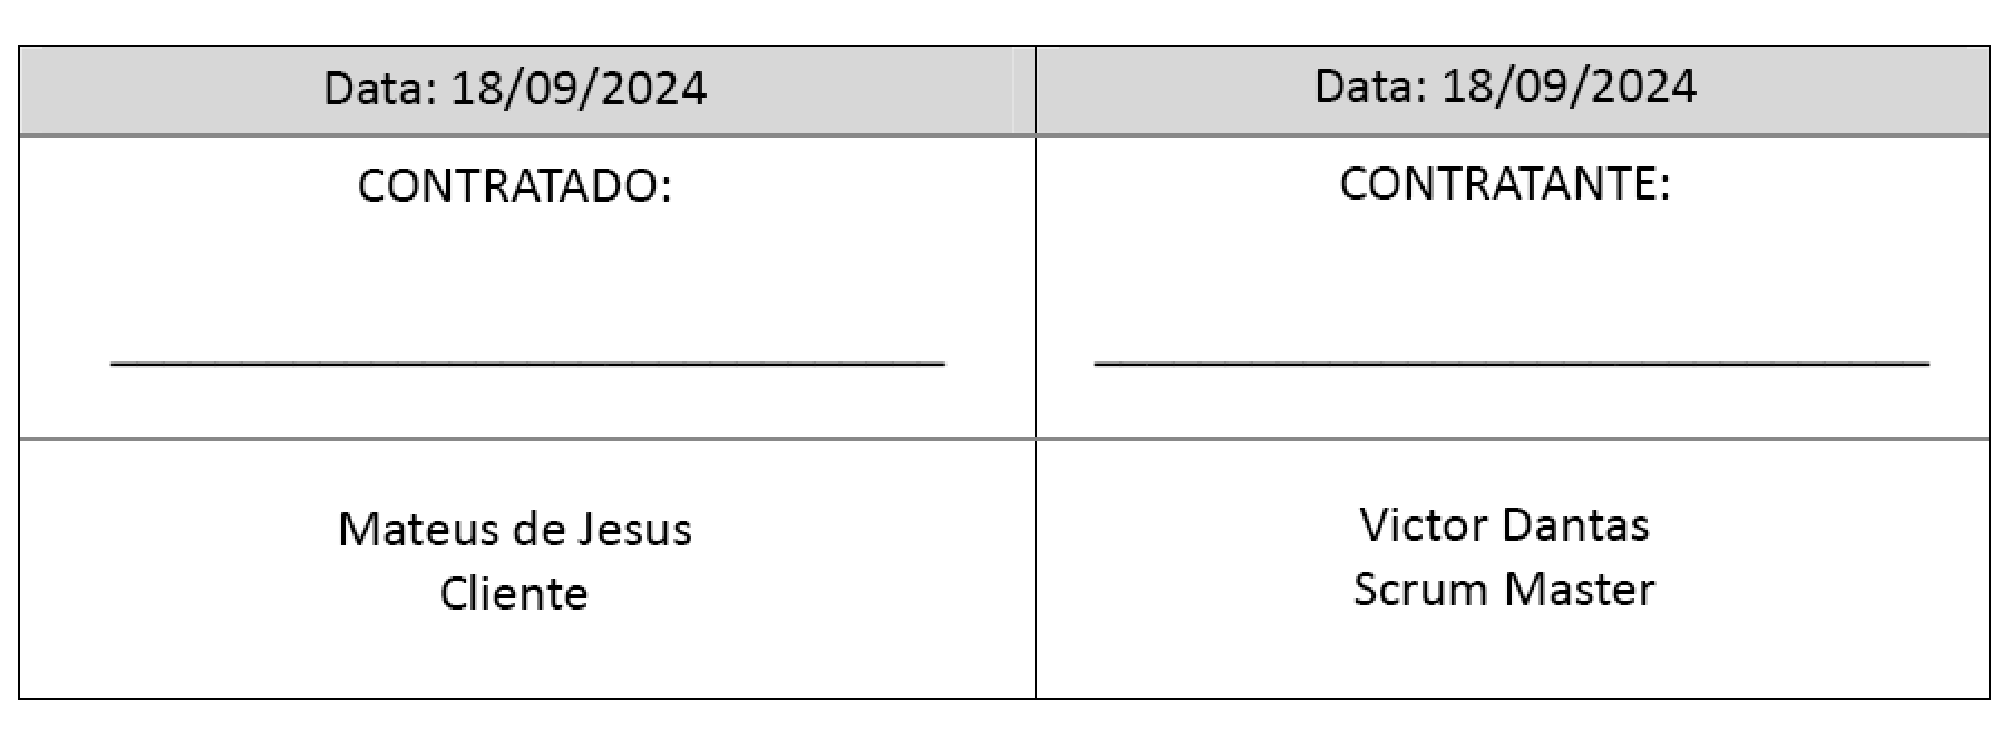
\includegraphics[width=1\textwidth]{PDFs/Assinatura.pdf} 
\end{center}